% Section 2: Method. All numbers are \jm... macros (make_macros.py + macros_sec_method.py). No hand-typed numbers.
% Labels used: sec:method, tab:worked, tab:oracle, tab:gates, tab:arbiter. Cross-references expected: sec:default, sec:guard, sec:waterfall, sec:validity.
\section{Method}\label{sec:method}

The method charges each wrong sentence to the party that could have prevented it.
A message is rendered through input channels that fix what the person supplied, a model writes a sentence, two extractor prompts label what the sentence commits to, and deterministic code turns the labels into a verdict.
The verdict is a function of the stored labels, the item specification and the channel, so a change of rule re-scores every stored output without a model call.
This section defines the units and the attribution rule (Sections~\ref{sec:m-items} and~\ref{sec:m-attr}), describes the extractor and its arbiter (Section~\ref{sec:m-judge}), and then validates each link of the chain: the checker against seeded and unseeded faults (Section~\ref{sec:m-oracle}), the extractor against human coders (Section~\ref{sec:m-gates}) and the arbiter against human coders (Section~\ref{sec:m-arbiter}).
The writer-grounded and expert instruments that the later sections use are defined in Section~\ref{sec:m-instruments}, and estimation in Section~\ref{sec:m-est}.
The harness follows the one first described in our concurrent archival and workshop papers~\cite{concurrent_se4all,concurrent_caleai}; the description here is complete for the results that follow.


\begin{figure}[t]
\centering
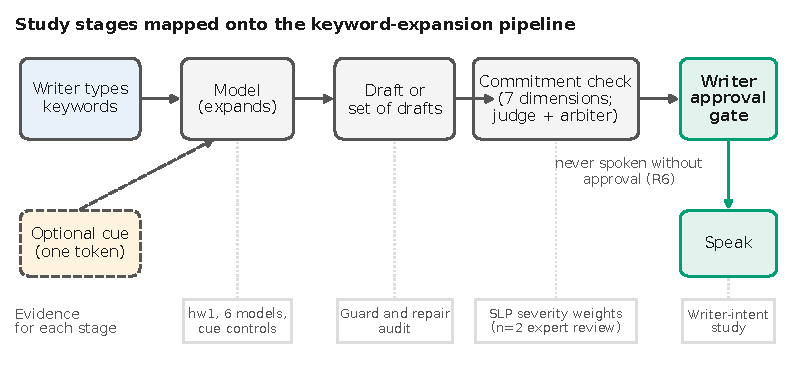
\includegraphics[width=\linewidth]{figs/fig1_pipeline.pdf}
\caption{Keyword-expansion pipeline with the approval gate, and where each study of this paper plugs in. A one-token cue is optional; nothing is spoken until the writer approves a draft (requirement R6, from the design consultants who use AAC). Schematic; no data.}\label{fig:pipeline}
\Description{Keyword-expansion pipeline with the approval gate, and where each study of this paper plugs in.}
\end{figure}

\subsection{Items, channels, models}\label{sec:m-items}

\paragraph{Families and dimensions.}
A \emph{family} is a minimal pair of source sentences that share their content words and differ on one \emph{critical} dimension: polarity, agent (who acts), certainty, speech act (statement, question or request), politeness, or time/quantity.
The two members of a pair, variants A and B, are rendered from the same keywords, so the keywords alone cannot tell them apart.
The extractor answers the family's critical question for every output and five general questions (polarity, speech act, agent, certainty, politeness), and it answers an added-content question.
These are the seven fields that the human checks below validate.

\paragraph{Channels.}
Each variant is shown to the model through five \emph{channels} that differ in how much of the message the person supplied.
\emph{Bare} gives the keywords only.
\emph{Non-critical} adds one content word that does not bear on the critical dimension and so matches the length of a cue.
\emph{Chip} adds the critical value as a one-token cue such as \texttt{[NOT]}, \texttt{[?]} or \texttt{[PLAIN]}.
\emph{All-chips} adds every cue the variant needs.
\emph{Full} gives the source sentence itself.
The chip is a probe of whether supplied information is used, not a proposed interface: its real cost depends on the access method, and a plain-word cue and an irrelevant-chip control are scored as separate channels (Section~\ref{sec:default}).
Table~\ref{tab:worked} shows one family through all five channels.

\paragraph{Evidence sets.}
The primary set is the human-written pairs (\emph{hw1}).
\jmhwWritersKept{} adult non-author classmates wrote \jmhwCand{} candidate minimal pairs and the keywords for them; three independent blind checkers per pair, who never saw model outputs, and a tie-break by one of six fixed checkers kept \jmhwKept{}, of which \jmhwFamilies{} are analysed after the exclusions stated in the hw1 report.
Each contrast rests on \jmhwWrMin{} to \jmhwWrMax{} writers.
Generation ran on all candidates before the checks, so dropped pairs are removed at analysis time.
A confirmation set of machine-written families with three pre-specified contrasts, and a development set used to build the prompts and codebook, are reported in the concurrent papers and enter here only where cited.

\paragraph{Models and prompt.}
Six models from \jmbreadthFamilies{} families write one sentence per request: Qwen2.5-7B-Instruct, Llama-3.1-8B-Instruct, Gemma-3-4B-it, Qwen2.5-14B-Instruct and Mistral-Nemo-12B-Instruct (4-bit GGUF, llama.cpp, local) and one API model, gpt-6.1-terra.
All use one fixed one-sentence prompt (\texttt{P0}) with greedy decoding; the prompt includes a short legend of the cues, and the no-legend arms of Section~\ref{sec:default} test whether the legend matters.
The hw1 run comprises \jmhwRequests{} requests.
A lite commercial Gemini model was added later under the same prompts as a seventh, machine-API replication, and is labelled as such where its rows appear.
Reissuing the same request reproduces the text for \jmndLocalMin{} to \jmndLocalMax{}\% of local requests and \jmndApiMin{} to \jmndApiMax{}\% of API requests, so every comparison is made on stored outputs for the same request and not on fresh draws.

\begin{table}[t]
\caption{One hw1 polarity family through the five channels, with the verdict each channel can give. Selection rule, declared before the draw: polarity families ordered by SHA-256 of the family id; the first family in which the bare output commits to the wrong value while the chip output matches; models in alphabetical order, then variant A, then B (here \jmexPolQual{} qualifying families; model \texttt{gemma3-4b}, variant B, target \emph{negated}; stored outputs and stored labels, not edited). Source sentence: ``The supervisor does not read my schedule.'' Rate the example represents: a committed bare output has the wrong value for the variant in \jmexPolWrong{}\% [\jmexPolWrongLo{}, \jmexPolWrongHi{}] of \jmexPolBareN{} bare rows (\jmexPolWriters{} writers), the design ceiling of a pair that shares one bare input, not a finding about models; given the chip, the output matches the target in \jmexPolChip{}\% [\jmexPolChipLo{}, \jmexPolChipHi{}] of \jmexPolChipN{} rows.}
\label{tab:worked}
\small
\setlength{\tabcolsep}{3pt}
\begin{tabular}{@{}l p{3.15cm} p{2.5cm} l l@{}}
\toprule
Channel & Input shown & Stored output & Label & Verdict\\
\midrule
Bare & \texttt{supervisor read} & The supervisor read. & affirmative & assumption (wrong value)\\
Non-critical & \texttt{supervisor read schedule} & The supervisor read the schedule. & affirmative & assumption (wrong value)\\
Chip & \texttt{[NOT] supervisor read} & The supervisor did not read. & negated & kept\\
All-chips & \texttt{[NOT] [TELL] [THEY] supervisor read} & The supervisor did not read. & negated & kept\\
Full & typed source sentence & The supervisor does not read my schedule. & negated & kept\\
\bottomrule
\end{tabular}
\end{table}

\subsection{Attribution by construction}\label{sec:m-attr}

Attribution is a property of the design, not a judgment about each output.
Let $C(x)$ be the set of dimensions whose value input $x$ fixes: the chip or the typed sentence fixes the critical dimension in the chip, all-chips and full channels, and nothing fixes it in the bare and non-critical channels.
For an output $y$ with extracted value $L_d(y)$ on dimension $d$ and meant value $s_d$:
\begin{itemize}
\item \textbf{Violation.} $d\in C(x)$ and $L_d(y)$ is not admissible for $s_d$. The model held the value and did not keep it. This is the only miss a checker can enforce.
\item \textbf{Assumption.} $d\notin C(x)$ and $L_d(y)$ is a committed value. The model chose a reading the input left open. An assumption is not a pass or a fail; we report its direction and share.
\item \textbf{Loss.} $d\notin C(x)$ and $L_d(y)\neq s_d$. The writer's value never reached the model. Loss and assumption are the same open-channel event seen from the interface (the value was lost) and from the model (it committed anyway); a loss is never charged as a violation.
\end{itemize}
Because the two variants of a pair share their open-channel input, a model that commits is wrong on exactly one of them, so paired match in an open channel has a ceiling that the design fixes; the quantity of interest is the gap between open and cue channels, not the open-channel rate.
The cue gain (chip minus non-critical) measures how much of the loss a cue recovers, and the irrelevant-chip control separates cue content from added tokens (Section~\ref{sec:default}).
A reference-fidelity score would charge the model for what the interface omitted; this rule does not.

Verdicts are computed in code from labels, the item specification and the channel, identically for treated and untreated outputs.
Plain assertion is honoured by emphatic certainty; unresolved critical labels are excluded and counted, not filled from either extractor prompt; and the added-content field is carried as a descriptive rate and enters no verdict rule.
Refusal and acceptance speech-act families are quarantined from every primary estimate because their predicate failed the oracle tests of Section~\ref{sec:m-oracle}.
The rule decides only whether explicit, text-level values are kept.
It does not judge fluency, reference resolution or whether the writer would accept the sentence; the writer-grounded analysis of Section~\ref{sec:waterfall} extends the attribution to that question.

\paragraph{Input honesty (R5).}
A failure cannot be charged to a model if the displayed input misstated the claim.
A validator therefore decodes the rendered input and rejects any cue that contradicts the source before generation.
Replayed on \jmtNineInputs{} chip inputs from the confirmation, composition and hw1 sets, it found \jmtNineConflicts{} conflicts; \jmtNineCompat{} inputs were verified compatible and \jmtNineUnknown{} (time chips and one long alias) lie outside its decoder, with \jmtNineGenCalls{} generation or judge calls.
Two defects found while building the harness, a relaxed acceptance predicate and an input-builder fallback, and the regression test each produced, are traced in the concurrent archival paper~\cite{concurrent_se4all}.

\subsection{Extractor, judge pair and arbiter}\label{sec:m-judge}

The extractor is gpt-6.1-sol at low reasoning effort, a model that is not among those under test.
It sees the output alone, not the source, the model or the channel, except for the added-content question, which also sees the visible input.
Two prompt variants, J1 and J2, differ in wording and option order.
On hw1 they labelled \jmhwUnits{} unique output units and agreed on the critical label for \jmhwJJCrit{}\% ($\kappa=\jmhwJJCritKappa{}$); the remaining \jmhwNeedArb{} units (\jmhwNeedArbShare{}\%) went to a blind arbiter.
The arbiter is a Claude model from a different family than the judge (claude-opus-5-5 for the confirmation set, claude-sonnet-5-5 for the other runs) and sees only the output text, the critical question and its options.
No J1 fallback enters a primary estimate, and every hw1 critical label is resolved by agreement or by the arbiter.
In the confirmation set the arbiter resolved \jmwcArbUnits{} units (\jmwcArbRows{} rows) after outcomes were known, blind to reference, model and condition, and the unknown-masked analysis is kept as a sensitivity analysis.
One tested model, gpt-6.1-terra, shares a vendor with the judge; its critical-label $\kappa$ against humans is reported with the other models in Section~\ref{sec:m-gates}.

\subsection{Testing the checker}\label{sec:m-oracle}

The checker is the extractor plus the verdict code; we test it as software, in the spirit of the test-oracle and mutation-analysis literature~\cite{weyuker1982nontestable,barr2015oracle,jia2011mutation}: an authorized change must pass and an unauthorized one must fail.
Table~\ref{tab:oracle} lists the evidence in the order of how far it is from our own hands.

\begin{table}[t]
\caption{Checker evidence. Authored rows use sentences we wrote or edited; the real-output rows seed one-value edits into stored hw1 outputs (seed \jmorrSeed{}; four booster mutants, which the contract tolerates, are excluded from the mutant counts); the last rows compare the judge's verdicts with the consensus of human coders on unedited outputs from held-out sets (Parts 10 and 13). Intervals are Wilson 95\%. None of the first two groups is an error rate on unedited outputs.}
\label{tab:oracle}
\small
\setlength{\tabcolsep}{3pt}
\begin{tabular}{@{}p{5.6cm} r@{}}
\toprule
Check & Result\\
\midrule
\multicolumn{2}{@{}l}{\emph{Authored inputs}}\\
Identity: unchanged source passes; false alarms & \jmorIdFaK{}/\jmorIdFaN{}\\
Scoped one-value mutants detected & \jmorMutK{}/\jmorMutN{}\\
Keyed challenge, mutants detected, production rule & \jmorKeyMutK{}/\jmorKeyMutN{}\\
\quad acceptance group only & \jmorKeyAccProdK{}/\jmorKeyAccProdN{}\\
\quad strict rule, no acceptance relaxation & \jmorKeyMutStrictK{}/\jmorKeyMutStrictN{}\\
Keyed challenge controls, false alarms & \jmorKeyCtlK{}/\jmorKeyCtlN{}\\
\midrule
\multicolumn{2}{@{}l}{\emph{Seeded edits of real outputs} (mutants caught; false alarms on \jmorrJFaN{} controls)}\\
Judge (J1, J2, arbiter) & \jmorrJMutK{}/\jmorrJMutN{} [\jmorrJMutLo{}, \jmorrJMutHi{}]\%; \jmorrJFaK{}/\jmorrJFaN{}\\
Surface lexicon (near-circular) & \jmorrSMutK{}/\jmorrSMutN{}; \jmorrSFaK{}/\jmorrSFaN{}\\
String overlap & \jmorrOMutK{}/\jmorrOMutN{}; \jmorrOFaK{}/\jmorrOFaN{}\\
\midrule
\multicolumn{2}{@{}l}{\emph{Unedited outputs, held-out human consensus} (precision; recall, \%)}\\
Violation verdict (\jmnatHoViolPos{} positives) & \jmnatHoViolP{} [\jmnatHoViolPLo{}, \jmnatHoViolPHi{}]; \jmnatHoViolR{} [\jmnatHoViolRLo{}, \jmnatHoViolRHi{}]\\
Preservation-failure verdict (\jmnatHoPresPos{} positives) & \jmnatHoPresP{} [\jmnatHoPresPLo{}, \jmnatHoPresPHi{}]; \jmnatHoPresR{} [\jmnatHoPresRLo{}, \jmnatHoPresRHi{}]\\
\bottomrule
\end{tabular}
\end{table}

\paragraph{Authored faults.}
An unchanged source injected as its own output must pass (the identity test), and a hand-written one-value change must be caught (scoped mutants).
A keyed challenge set of controls and one-feature mutants, with keys hashed before the first extractor call, has four groups: acceptance, embedded actors, question versus request, and mitigated requests.
The production rule detects \jmorKeyMutK{} of \jmorKeyMutN{} keyed mutants; the strict rule without the acceptance relaxation detects \jmorKeyMutStrictK{} of \jmorKeyMutStrictN{}, and the relaxation accounts for the difference, using up the pre-specified miss tolerance.
This is why refusal and acceptance families are quarantined: removing a false alarm from the acceptance predicate removed fault sensitivity.

\paragraph{Faults in real outputs.}
Hand-written faults are easy.
We therefore seeded \jmorrNAll{} one-value mutants into stored hw1 outputs that the checker had scored as preserving, with operators for each dimension (negation insertion and removal, speech-act flips, agent swaps, hedge insertion and removal, politeness addition and removal, time shifts), and drew \jmorrJFaN{} meaning-preserving surface edits as controls.
The judge caught \jmorrJMutK{} of \jmorrJMutN{} mutants with \jmorrJFaK{} false alarms, and no unresolved rows.
A surface lexicon of negation, hedge, politeness, tense and question cues scored \jmorrSMutK{} of \jmorrSMutN{} with \jmorrSFaK{} false alarms, and string overlap \jmorrOMutK{} of \jmorrOMutN{} with \jmorrOFaK{} false alarms.
The lexicon matches the cues the operators insert, so its score shows that the operators are lexically shallow and not that a lexicon is an adequate checker; the judge's advantage shows mainly on controls.

\paragraph{Faults nobody seeded.}
Seeded faults are faults we thought of.
The test on unedited outputs uses the human-coded sets of Section~\ref{sec:m-gates}: on the two sets not used to build the codebook, the judge's violation verdicts have precision \jmnatHoViolP{}\% and recall \jmnatHoViolR{}\% against the human consensus (\jmnatHoViolPos{} positives in \jmnatHoUnitsViol{} verdicts), and its preservation-failure verdicts \jmnatHoPresP{}\% and \jmnatHoPresR{}\% (Table~\ref{tab:oracle}).
Each set has few positives, so the intervals are wide.
Machine agreement is not validation: on a keyed challenge sentence, ``I can't wait to go to the party,'' the judge and the machine panel read \emph{negated}, a known blind spot for idiomatic negation, which is why no claim here rests on machine-panel agreement.

\subsection{Validating the extractor against human coders}\label{sec:m-gates}

Four human gates compare the extractor's final label with the plurality label of trained human coders on stored outputs (Table~\ref{tab:gates}).
Coders labelled the same fields from the stored output with the same options as the judge, after being taught the same codebook with practice items.
The development gate (H7) used the extraction inventory from which the codebook was built.
round~10 coded fresh outputs from the confirmation, composition and guard-transfer runs; round~12 coded outputs for keywords that other annotators typed for stored messages; round~13 coded outputs for the human-written pairs.
Rounds~10, 12 and 13 are therefore later checks on outputs the harness was not developed on.
Each gate samples stored outputs by a seeded draw and keeps a seeded quarter for calibration; $\kappa$ is computed on the remaining test split.
The stored rule excludes ties and unsure answers from the reference; the strict rule counts them as disagreement, and the table reports the strict rule with a family-cluster bootstrap interval.

\begin{table}[t]
\caption{Extractor against human coders, test split (Cohen's $\kappa$). Strict rule: ties and unsure answers count as disagreement; intervals are family-cluster bootstrap 95\%. Human--human and judge--human $\kappa$ are computed on the same items for the critical field. All coders were adult non-author classmates. Added content is the weakest field in Parts 10 and 13.}
\label{tab:gates}
\footnotesize
\setlength{\tabcolsep}{2.5pt}
\begin{tabular}{@{}l r r r l r r r r@{}}
\toprule
Gate & Coders & Items (test) & Stored $\kappa$ & Strict critical $\kappa$ [CI] & Hum--hum & Judge--hum & Speech act & Added\\
\midrule
H7 (development) & \jmhgHSevenCoders{} & \jmhgHSevenSampled{} (\jmhgHSevenTest{}) & \jmhgHSevenCritRZero{} & \jmhgHSevenCrit{} [\jmhgHSevenCritLo{}, \jmhgHSevenCritHi{}] & \jmhgHSevenHH{} & \jmhgHSevenJH{} & \jmhgHSevenAct{} & \jmhgHSevenAdded{}\\
Round 10 (fresh runs) & \jmhgPTenCoders{} & \jmhgPTenSampled{} (\jmhgPTenTest{}) & \jmhgPTenCritRZero{} & \jmhgPTenCrit{} [\jmhgPTenCritLo{}, \jmhgPTenCritHi{}] & \jmhgPTenHH{} & \jmhgPTenJH{} & \jmhgPTenAct{} & \jmhgPTenAdded{}\\
Round 12 (typed keywords) & \jmhgPTwelveCoders{} & \jmhgPTwelveSampled{} (\jmhgPTwelveTest{}) & \jmhgPTwelveCritRZero{} & \jmhgPTwelveCrit{} [\jmhgPTwelveCritLo{}, \jmhgPTwelveCritHi{}] & \jmhgPTwelveHH{} & \jmhgPTwelveJH{} & \jmhgPTwelveAct{} & \jmhgPTwelveAdded{}\\
Round 13 (human-written pairs) & \jmhgPThirteenCoders{} & \jmhgPThirteenSampled{} (\jmhgPThirteenTest{}) & \jmhgPThirteenCritRZero{} & \jmhgPThirteenCrit{} [\jmhgPThirteenCritLo{}, \jmhgPThirteenCritHi{}] & \jmhgPThirteenHH{} & \jmhgPThirteenJH{} & \jmhgPThirteenAct{} & \jmhgPThirteenAdded{}\\
\bottomrule
\end{tabular}
\end{table}

On the critical field the extractor's strict-rule $\kappa$ is at least \jmhgCritMin{} in every gate, with the lowest lower interval bound at \jmhgCritLoMin{}, against a pre-specified gate of \jmhgGate{}.
In every gate the judge--human $\kappa$ sits just below the human--human $\kappa$ on the same items, so the extractor is close to, not above, the agreement that two people reach.
By model, the critical-field $\kappa$ on the development gate lies between \jmhgHSevenModelMin{} and \jmhgHSevenTerra{} (gpt-6.1-terra, $n=\jmhgHSevenTerraN{}$).
The added-content field is the exception: its $\kappa$ is \jmhgPTenAdded{} on round~10 and \jmhgPThirteenAdded{} on round~13 (J1--J2 agreement on hw1 is $\kappa=\jmhwJJAddedKappa{}$), so no verdict or estimate here is built on it.
These gates cover untreated outputs and the codebook is shared between humans and judge; they validate extraction of explicit markers, not repaired or rewritten text, which the audits of Section~\ref{sec:m-instruments} address.

\subsection{Validating the arbiter against human coders (arbiter check)}\label{sec:m-arbiter}

The arbiter decides every unit on which the two extractor prompts disagree, so it carries the hardest labels.
The arbiter check asks people to code exactly those units.
Each of \jmpOneNinePeople{} annotators coded a seeded set of items, two coders per item.
The key holds \jmpOneNineArbItems{} arbiter units, stratified by run and by the precedent the arbiter applied (for example, ``I want X, please'' is a request), on every one of which J1 and J2 disagreed, and \jmpOneNineCanYouItems{} ``Can you\ldots?'' or ``Could you\ldots?'' outputs for which the codebook example was hidden.
Coders did not receive items from their own pairs or keyword sets.
Of the \jmpOneNineArbExpected{} codings on arbiter units, \jmpOneNineArbLabelledN{} carried a label; the remaining \jmpOneNineArbUnlabelledShare{}\% were unsure or blank and are excluded, not counted as disagreement, so the agreement below is conditional on a person committing to a label.
Intervals are Wilson and descriptive, because codings are not independent.

\begin{table}[t]
\caption{Humans against the arbiter and each judge prompt on the \jmpOneNineArbItems{} arbiter units (\jmpOneNineCodings{} labelled codings, all units ones on which J1 and J2 disagreed). The arbiter sided with J1 on \jmpOneNineSidedJOne{} units, with J2 on \jmpOneNineSidedJTwo{} and with neither on \jmpOneNineSidedNeither{}.}
\label{tab:arbiter}
\small
\begin{tabular}{@{}l r r@{}}
\toprule
Reference & Agreement with humans (\%) [95\% CI] & Cohen's $\kappa$\\
\midrule
Arbiter & \jmpOneNineAgreeArb{} [\jmpOneNineAgreeArbLo{}, \jmpOneNineAgreeArbHi{}] & \jmpOneNineKappaArb{}\\
J1 & \jmpOneNineAgreeJOne{} [\jmpOneNineAgreeJOneLo{}, \jmpOneNineAgreeJOneHi{}] & \jmpOneNineKappaJOne{}\\
J2 & \jmpOneNineAgreeJTwo{} [\jmpOneNineAgreeJTwoLo{}, \jmpOneNineAgreeJTwoHi{}] & \jmpOneNineKappaJTwo{}\\
\bottomrule
\end{tabular}
\end{table}

Humans side with the arbiter more often than with either prompt (Table~\ref{tab:arbiter}).
They match the arbiter on \jmpOneNineMatchJOneSide{}\% [\jmpOneNineMatchJOneSideLo{}, \jmpOneNineMatchJOneSideHi{}] of codings where it sided with J1 and \jmpOneNineMatchJTwoSide{}\% [\jmpOneNineMatchJTwoSideLo{}, \jmpOneNineMatchJTwoSideHi{}] where it sided with J2, so the arbiter is not simply the more frequent prompt.
Where both coders of an item gave a label, they agree with each other on \jmpOneNineHHAgree{}\% (\jmpOneNineHHItems{} items, $\kappa=\jmpOneNineHHKappa{}$); \jmpOneNineSplit{} arbiter items split their coders.
The disagreements with the arbiter concentrate in a few precedent tags with few items each (for example, ``I want X, please'' and ``I tell you to\ldots''); the supplement lists them with their counts, and we do not pool them away.
On the codebook rule that ``Can you\ldots?'' is a request, \jmpOneNineCanYouRequest{}\% [\jmpOneNineCanYouRequestLo{}, \jmpOneNineCanYouRequestHi{}] of \jmpOneNineCanYouLabelled{} labelled codings chose request or command, from coders who had not been shown the rule; the alternative coding as a question is not what people do.
\paragraph{What the exclusion and the dependence do to the estimate.}
Excluding unsure or blank codings matters: if every one of the \jmpOneNineSensUnsure{}\% unlabelled codings on the arbiter units (\jmpOneNineSensLabelled{} labelled of \jmpOneNineSensTotal{}) were counted as a disagreement, agreement with the arbiter would be \jmpOneNineSensLowerBound{}\%, so the \jmpOneNineAgreeArb{}\% is an agreement among codings where a person committed, and these are the units on which two prompts already disagreed.
Codings share items and coders, so we resampled items as clusters: the interval is \jmpOneNineSensBootLo{} to \jmpOneNineSensBootHi{}\%, close to the descriptive Wilson interval.
Dropping any one coder moves agreement only between \jmpOneNineSensLooMin{}\% and \jmpOneNineSensLooMax{}\%.
Per-coder agreement is far noisier (\jmpOneNineSensCoderMin{} to \jmpOneNineSensCoderMax{}\% over the \jmpOneNineSensCoderN{} coders with at least five labelled codings), and the \jmpOneNineSensCoderPairs{} coder pairs share only a few items each, so a kappa per coder pair is not estimable; the only pair-level statistic we report is the human--human agreement on items where both coders labelled.
We therefore call the arbiter \emph{checked against human codings of the disputed units}, and do not call it validated in general: the evidence is a moderate-sized check of the hardest units, with a stated attrition.

The consequence for the method is fixed in advance of every analysis: arbiter labels are the reference for disputed units, no J1 fallback enters a primary estimate, and the effect of recoding ``Can you\ldots?'' is reported next to the primary estimate (Section~\ref{sec:default}).

\subsection{Writer-grounded and expert instruments}\label{sec:m-instruments}

Four further instruments supply the human evidence of later sections; their results are not repeated here.
\textbf{Repair-usability audit (blind three-rater audit).}
\jmpOneSevenItemsPerArm{} repaired texts and \jmpOneSevenItemsPerArm{} controls, plus a secondary arm of the pre-repair originals, were rated blind to arm by \jmpOneSevenRaters{} raters, \jmpOneSevenPerItem{} per item.
The primary endpoint, the item-level consensus ``usable'' (strict majority of its raters), and the decision rule for repaired minus control were frozen in the repository before any rating was returned; the rule and its three outcomes are stated in the protocol and applied unchanged.
\textbf{Writer-intent check (the writer-intent study).}
Each of the \jmpOneEightWriters{} writers rated \jmpOneEightPerWriter{} outputs for their own pairs, half from the bare channel and half from the chip channel, choosing which variant the sentence says (A, B, something else, unclear) and whether they would accept it as their message.
The judge labels the critical dimension only, while the writer judges the whole message; the instrument is writer-intent agreement and not validation by AAC users.
\textbf{Expert annotators.}
Two anonymous speech-language pathologists rated the seriousness of each kind of silent meaning change on an anchored scale and rated stored outputs blind to arm; the result is an expert review by two raters, not a population estimate.
\textbf{Design consultants.}
Two paid design consultants who use AAC reviewed the requirements and example outputs; every suggestion and the resulting change or non-change is logged, and we report requirement changes, not the consultants' experiences.
Annotators were adult non-author university classmates who consented and were paid (payment and food); the two expert annotators and two consultants were paid under written agreements.
No institutional review determination was sought.

\subsection{Estimation}\label{sec:m-est}

Contrasts are differences of row-weighted means over targets, where a target is one (item, model, channel, variant) outcome and the model roster is fixed.
Intervals are pointwise 95\% percentile intervals from \jmhwBootN{} cluster resamples (seed \jmhwSeed{}): writers are the clusters for hw1 and construction clusters for the confirmation set.
Proportions of codings use Wilson intervals, and $\kappa$ intervals use family-cluster bootstrap.
With \jmhwWrMin{} to \jmhwWrMax{} writers per contrast, the writer-cluster intervals are optimistic, and we claim direction and consistency across writers, not interval width.
No interval corrects for exploratory selection or for extractor error beyond the validation above.
Analyses were pre-specified and git-timestamped; we do not call them pre-registered, and the public hash deposits post-date the confirmation freeze and do not certify it.
Numbers in tables and text are generated from the stored analysis files by a script, and the verdict rule can be re-run on stored labels with no model call.
